\documentclass[10pt,tikzpicture,notheorems]{beamer}
\usepackage{animate}
\usepackage[backend=bibtex,firstinits=true]{biblatex}
\usepackage{graphicx}
\usepackage{amsfonts}
\usepackage{amsthm}
\usepackage{etoolbox}
\usepackage{filecontents}
\usepackage{mathtools}
\usepackage{ragged2e}
\justifying

\usepackage{changepage}
\usepackage{xcolor}
\definecolor{pythongreen}{RGB}{106,160,93}
\definecolor{pythonorange}{RGB}{217,118,27}
\definecolor{pythongray}{RGB}{140,139,135}
\usepackage{listings}
\definecolor{codegreen}{rgb}{0.43,0.57,0.49}
\definecolor{codegray}{rgb}{0.5,0.5,0.5}
\definecolor{codepurple}{rgb}{0.4,0.43,0.58}
\definecolor{codeorange}{rgb}{0.70,0.57,0.51}
%\definecolor{backcolour}{rgb}{0.95,0.95,0.92}
\definecolor{backcolour}{rgb}{0.11,0.12,0.13}
\definecolor{plaincode}{rgb}{0.69,0.72,0.75}

\lstdefinestyle{mystyle}{
    backgroundcolor=\color{backcolour},
    commentstyle=\color{codegreen},
    keywordstyle=\color{codeorange},
    numberstyle=\tiny\color{codegray},
    stringstyle=\color{codepurple},
    basicstyle=\ttfamily\footnotesize\color{plaincode},
    breakatwhitespace=false,
    breaklines=true,
    captionpos=b,
    keepspaces=true,
    numbers=left,
    numbersep=5pt,
    showspaces=false,
    showstringspaces=false,
    showtabs=false,
    tabsize=2
}

\lstset{style=mystyle}


\setbeamerfont{quote}{shape=\upshape,family=\ttfamily}


%\inserttheoremnumber


\usetheme{Warsaw}
\usecolortheme{whale}

\let\Tiny=\tiny

\hypersetup{bookmarksdepth=4,bookmarksnumbered=true,bookmarksopen=true}

\beamertemplatenavigationsymbolsempty

\setbeamersize{text margin left=5mm,text margin right=5mm}

\setbeamertemplate{qed symbol}{\rule{0.2cm}{0.2cm}}
\setbeamertemplate{theorems}[numbered]
\setbeamertemplate{caption}[numbered]
%\setbeamertemplate{enumerate item}{(\roman{enumi})}

\setbeamertemplate{background canvas}[vertical shading][bottom=white!10,top=blue!10]
\usefonttheme[onlymath]{serif}

\makeatletter
\renewcommand\eqref[1]{%
  \textup{\usebeamercolor[fg]{structure}\tagform@{\ref{#1}}}%
}

%\DefineBibliographyStrings{english}{%
%  references = {Kaynak\c{c}a},
%  and = {ve},
%  andothers = {vd.}
%}

\DefineBibliographyExtras{english}{
  \let\finalandcomma=\empty
}

%\undef{\theorem}
\newtheorem{theorem}{Theorem}
\newtheorem{corollary}{Corollary}

%\undef{\lemma}
\newtheorem{lemma}{Lemma}

%\undef{\example}
\theoremstyle{example}
\newtheorem{example}{Example}

%\undef{\definition}
\theoremstyle{definition}
\newtheorem{definition}{Definition}
\newtheorem{property}{Property}

%

%http://tex.stackexchange.com/a/123992/9955
\makeatletter
\def\th@remark{%
    \normalfont % body font
    \setbeamercolor{block title alert}{use=alerted text,fg=white,bg=alerted text.fg!75!black}
    \setbeamercolor{block body alert}{parent=normal text,use=block title alerted,bg=block title alerted.bg!10!bg}
    \def\inserttheoremblockenv{alertblock}
  }
\makeatother

\theoremstyle{remark}
\newtheorem{remark}{Remark}

%\setbeamertemplate{bibliography item}[text]

\setbeamertemplate{bibliography item}{%
  \ifboolexpr{test {\ifentrytype{book}} or test {\ifentrytype{thesis}}}
    {\setbeamertemplate{bibliography item}[book]}
    {\ifentrytype{online}
       {\setbeamertemplate{bibliography item}[online]}
       {\setbeamertemplate{bibliography item}[article]}}%
  \usebeamertemplate{bibliography item}
}

\defbibenvironment{bibliography}
  {\list{}
     {\settowidth{\labelwidth}{\usebeamertemplate{bibliography item}}%
      \setlength{\leftmargin}{\labelwidth}%
      \setlength{\labelsep}{\biblabelsep}%
      \addtolength{\leftmargin}{\labelsep}%
      \setlength{\itemsep}{\bibitemsep}%
      \setlength{\parsep}{\bibparsep}}}%
  {\endlist}
  {\item}

%http://tex.stackexchange.com/questions/28760/custom-beamer-blocks
\newenvironment<>{refblock}[1]{%
  \begin{actionenv}#2%
      \def\insertblocktitle{#1}%
      \par%
      \mode<presentation>{%
       \setbeamercolor{block title}{fg=white,bg=orange!20!black}
       \setbeamercolor{block body}{fg=black,bg=yellow!20}
     }%
      \vfill
      \usebeamertemplate{block begin}}
    {\par\usebeamertemplate{block end}\end{actionenv}}

\newenvironment<>{tableblock}[1]{%
  \begin{actionenv}#2%
      \def\insertblocktitle{#1}%
      \par%
      \mode<presentation>{%
    \setbeamercolor{block title}{fg=white,bg=orange}
    \setbeamercolor{block body}{fg=black,bg=orange!20}
     }%
      \vfill
      \usebeamertemplate{block begin}}
    {\par\usebeamertemplate{block end}\end{actionenv}}

\renewcommand*{\newunitpunct}{\addcomma\space}

\DeclareFieldFormat[article]{title}{#1}
\DeclareFieldFormat[article]{citetitle}{#1}
\DeclareFieldFormat[article]{volume}{\mkbibbold{#1}} %\bibstring{volume}\,{#1}
\DeclareFieldFormat[article]{number}{\bibstring{number}\thinspace{#1}}
\DeclareFieldFormat[article]{year}{\mkbibparens{#1}}
\DeclareFieldFormat[article]{pages}{#1}

\DeclareFieldFormat[book]{title}{#1} %\mkbibemph{#1}
\DeclareFieldFormat[book]{citetitle}{#1} %\mkbibemph{#1}
\DeclareFieldFormat[book]{pages}{#1}
\DeclareFieldFormat[book]{volume}{\bibstring{volume}\thinspace{#1}}

\DeclareFieldFormat[incollection]{title}{#1}
\DeclareFieldFormat[incollection]{citetitle}{#1}
\DeclareFieldFormat[incollection]{booktitle}{#1} %\mkbibemph{#1}
\DeclareFieldFormat[incollection]{pages}{#1}

\DeclareFieldFormat[inproceedings]{title}{#1}
\DeclareFieldFormat[inproceedings]{citetitle}{#1}
\DeclareFieldFormat[inproceedings]{booktitle}{#1} %\mkbibemph{#1}
\DeclareFieldFormat[inproceedings]{pages}{#1}

\DeclareFieldFormat[thesis]{title}{#1} %\mkbibemph{#1}
\DeclareFieldFormat[thesis]{citetitle}{#1} %\mkbibemph{#1}
\DeclareFieldFormat[thesis]{pages}{#1}
\DeclareFieldFormat[thesis]{annote}{#1}
\DeclareFieldFormat[online]{title}{#1}
\DeclareFieldFormat[online]{citetitle}{#1}
\DeclareFieldFormat[online]{url}{\url{#1}} %\mkbibacro{URL}\addcolon\space\url{#1}


\renewbibmacro{in:}{}


\renewbibmacro*{journal+issuetitle}{%
  \printfield{journaltitle}%
  \setunit*{\space}%
  \printfield{volume}%
  \setunit*{\space}%
  \printfield{year}% Added
  \setunit*{\addcomma\space}%
  \printfield{number}%
  \newunit
}

\renewbibmacro*{publisher+location+date}{%
    \printlist{publisher}%
    \setunit*{\addcomma\space}%
    \printlist{location}%
    \setunit*{\addcomma\space}%
    \printdate%
}

\newenvironment{referencelist}{%
 \setbeamerfont{description item}{size=\tiny}
 \setbeamersize{description width=0cm}
 \begin{description}\tiny}{\end{description}
}

\newenvironment{articleitem}[1]{%
 {\usebeamercolor[fg]{bibliography entry author}\usebeamerfont{bibliography entry author}\cite{#1}}
 {\usebeamercolor[fg]{bibliography entry author}\usebeamerfont{bibliography entry author}\citeauthor{#1},}
 {\usebeamercolor[fg]{bibliography entry title}\usebeamerfont{bibliography entry title}\citetitle{#1},}
 {\usebeamercolor[fg]{bibliography entry location}\usebeamerfont{bibliography entry location}\citefield{#1}[article]{journaltitle}, \citefield{#1}[article]{volume} \citeyear{#1}, \citefield{#1}[article]{number}, \citefield{#1}{pages}.}
}


\newenvironment{bookitem}[1]{%
 {\usebeamercolor[fg]{bibliography entry author}\usebeamerfont{bibliography entry author}\cite{#1}}
 {\usebeamercolor[fg]{bibliography entry author}\usebeamerfont{bibliography entry author}\citeauthor{#1},}
 {\usebeamercolor[fg]{bibliography entry title}\usebeamerfont{bibliography entry title}\citetitle{#1},}
 {\usebeamercolor[fg]{bibliography entry location}\usebeamerfont{bibliography entry location}\citelist{#1}{publisher}, \citeyear{#1}.}
}


\newenvironment{thesisitem}[1]{%
 {\usebeamercolor[fg]{bibliography entry author}\usebeamerfont{bibliography entry author}\cite{#1}}
 {\usebeamercolor[fg]{bibliography entry author}\usebeamerfont{bibliography entry author}\citeauthor{#1},}
 {\usebeamercolor[fg]{bibliography entry title}\usebeamerfont{bibliography entry title}\citetitle{#1},}
 {\usebeamercolor[fg]{bibliography entry location}\usebeamerfont{bibliography entry location}\citefield{#1}[thesis]{type}, \citelist{#1}{institution}, \citeyear{#1}.}
}

\newenvironment{webitem}[1]{%
 {\usebeamercolor[fg]{bibliography entry author}\usebeamerfont{bibliography entry author}\cite{#1}}
 {\usebeamercolor[fg]{bibliography entry author}\usebeamerfont{bibliography entry author}\citeauthor{#1},}
 {\usebeamercolor[fg]{bibliography entry title}\usebeamerfont{bibliography entry title}\citetitle{#1},}
 {\usebeamercolor[fg]{bibliography entry location}\usebeamerfont{bibliography entry location}\citeurl{#1}.}
}

%\addbibresource{\jobname.bib}

\DeclareMathOperator{\Log}{Log}

\newcommand{\dd}{\mathrm{d}}
\newcommand{\dD}{\mathrm{D}}
\newcommand{\ef}{\mathrm{e}}
\newcommand{\imn}{\mathrm{i}}
\newcommand{\Lop}{\mathrm{L}}
\newcommand{\Iop}{\mathrm{I}}

\newcommand{\cnt}[1]{\mathrm{C}^{#1}}

\newcommand{\N}{\mathbb{N}}
\newcommand{\R}{\mathbb{R}}
\newcommand{\Z}{\mathbb{Z}}
\newcommand{\C}{\mathbb{C}}

\renewcommand{\Re}{\operatorname{Re}}
\renewcommand{\Im}{\operatorname{Im}}

\renewcommand*{\thefootnote}{\fnsymbol{footnote}}

\title[{\makebox[.45\paperwidth]{Mathematical Modeling of a Three Axis Robotic Arm \hfill%
\insertframenumber/\inserttotalframenumber}}]%
{Mathematical Modeling of a\\Three Axis Robotic Arm}

\titlegraphic{
\includegraphics[width=0.15\textwidth]{deulogo.eps}}

\author[U.~\"{O}zen, A.~\"{O}zdoğan]{Umut \"{O}zen, Aleyna \"{O}zdoğan}

\institute{Department of Mathematics,\\
Dokuz Eyl\"{u}l University\\
\textit{Supervisor: Prof. Dr.~Ba\c{s}ak Karpuz}}

\date{2024--2025 -- Spring Semester}

\begin{document}

\begin{frame}
\titlepage
\end{frame}

%

\begin{frame}{Abstract}
\frametitle{Abstract}

\begin{block}{Abstract}
This presentation models and simulates the spatial motion of a three-degree-of-freedom robotic arm using Python. Joint coordinates are calculated based on link lengths ($L_1$, $L_2$) and joint angles ($\theta$, $\phi_1$, $\phi_2$) through trigonometric expressions. The geometric and trigonometric conditions for the arm’s endpoint to reach a target surface (e.g., a whiteboard) are analyzed, including valid joint angle ranges. Vector analysis, trigonometric transformations, and the law of cosines are employed, and the results are visualized and tested in Python. The project offers a theoretical and practical approach to solving inverse kinematics problems in robotics.
\end{block}

\end{frame}

%

\begin{frame}{Outline of the Talk }
\begin{enumerate}
  \item \textbf{Introduction and Applications}
  \begin{itemize}
    \item Real-world applications of 3 variable robotic arms\\
    (e.g., assembly lines, surgery, 3D printing, education)
    \item Motivation: Need for precise control in spatial environments
  \end{itemize}
  
  \item \textbf{Problem Definition}
  \begin{itemize}
    \item What is spatial positioning?
    \item Why modeling robotic arm kinematics is challenging and important
  \end{itemize}

  \item \textbf{Mathematical Representation of the Robotic Arm}
  \begin{itemize}
    \item Definition of link lengths ($L_1$, $L_2$) and joint angles ($\theta$, $\phi_1$, $\phi_2$)
    \item Description of coordinate system and base point ($x_0$, $y_0$, $z_0$)
  \end{itemize}
\end{enumerate}
\end{frame}

\begin{frame}{Outline of the Talk }
\begin{enumerate}
  \setcounter{enumi}{3}
  \item \textbf{Forward and Inverse Kinematics}
  \begin{itemize}
    \item Computing joint positions ($x_1$, $y_1$, $z_1$) and end-effector ($x_2$, $y_2$, $z_2$)
    \item Deriving inverse kinematic expressions for $\theta$, $\phi_1$, $\phi_2$
  \end{itemize}

  \item \textbf{Geometric and Trigonometric Constraints}
  \begin{itemize}
    \item Applying the law of cosines and triangle relationships
    \item Constraints for reaching a target (e.g., whiteboard surface)
  \end{itemize}

  \item \textbf{Python-Based Simulation and Visualization}
  \begin{itemize}
    \item Implementation of kinematic model in Python
    \item 3D graphical representation and animation of the robotic arm
  \end{itemize}
\end{enumerate}
\end{frame}

%

\section{Applications of Three Axis Robotic Arm}
\subsection{Applications Example of Two-Link Arms}
\begin{frame}
\frametitle{\insertsectionhead}

\begin{itemize}
  \item \textbf{Assembly Lines:} 3D positioning and precise assembly of components.
  \item \textbf{Welding and Painting Applications:} Performing tasks at complex angles.
  \item \textbf{Surgical Robots:} Medical operations requiring precise, multi‐axis movements.
  \item \textbf{3D Printing and CNC Machining:} Executing complex toolpaths in manufacturing.
  \item \textbf{Research and Education:} Used in advanced robotics control and kinematic studies.
\end{itemize}
\end{frame}

%%

\subsection{Application Photos of Two-Link Arms}
\begin{frame}
\frametitle{Applications of Two-Arm Robotic Systems}
\framesubtitle{Excavation and Industrial Robotics}

\begin{figure}
  \centering
  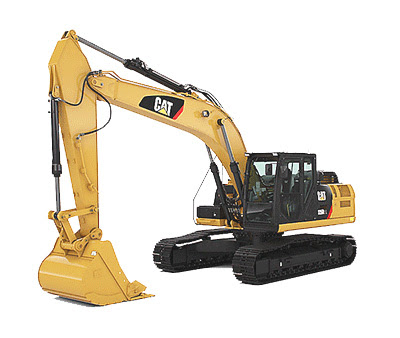
\includegraphics[width=0.45\textwidth]{excavator.jpg}
  \hfill
  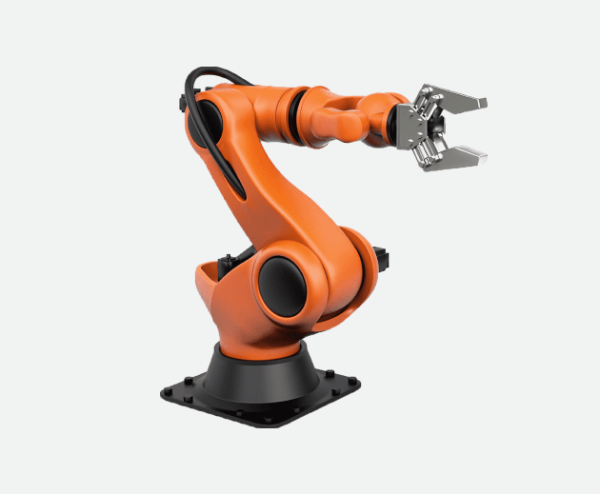
\includegraphics[width=0.45\textwidth]{poster_foto_2.png}
\end{figure}

\vspace{0.5em}
\centering
{\small \hfill Excavator system \hfill \textbar{} \hfill Industrial robot arm \hfill }

\end{frame}


%%

\section{Problem Statement}
\subsection{Kinematic Modeling of a 3 Variable Robotic Arm}

\begin{frame}
\frametitle{\insertsectionhead}
\framesubtitle{\insertsubsectionhead}

The precise control and spatial positioning of robotic arms with multiple variables present significant challenges in robotics.

\vspace{1em}

Modeling the kinematics of a three-axis robotic arm mathematically is essential for understanding its movement, enabling accurate targeting and manipulation within a 3D workspace.

\vspace{1em}

This project aims to develop a comprehensive mathematical model and simulation framework to solve the forward and inverse kinematics problems for such robotic arms, ensuring efficient and reliable operation in real-world applications.

\end{frame}

%%
\section{Representation of Robot Arm Angles and Coordinates}

\begin{frame}
\frametitle{\insertsectionhead}
\framesubtitle{\insertsubsectionhead}

\begin{figure}
  \centering
  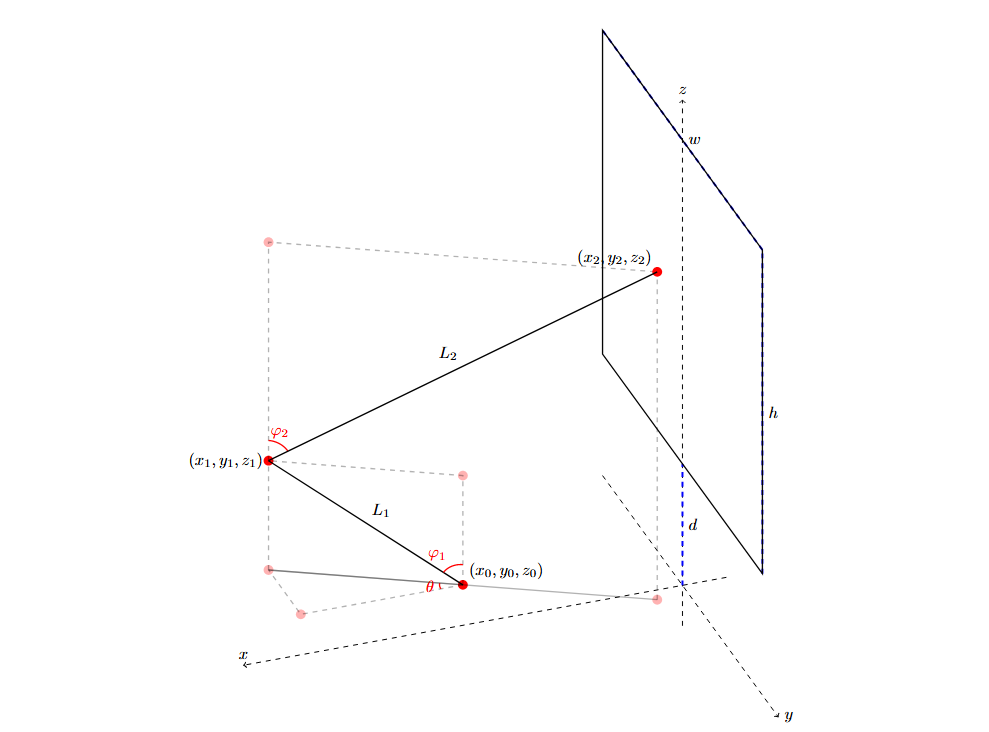
\includegraphics[width=0.7\textwidth]{mainphoto.png}
\end{figure}

\end{frame}


%%

\section{Mathematical Representation of the Robotic Arm}
\subsection{Link Lengths and Joint Angles}

\begin{frame}
\frametitle{\insertsectionhead}
\framesubtitle{\insertsubsectionhead}

Let $(x_0, y_0, z_0)$ denote the base point of the robotic arm.  
Let $L_1$ and $L_2$ be the lengths of the first and second links, respectively.  

\begin{itemize}
  \item $\phi_1$ is the angle between link $L_1$ and the $z$-axis.
  \item $\phi_2$ is the angle between link $L_2$ and the $z$-axis.
  \item $\theta$ is the angle between the $x$-axis and the $xy$-projection of $L_1$.
\end{itemize}

\end{frame}


%%

\subsection{Forward Kinematic Equations}

\begin{frame}
\frametitle{\insertsectionhead}
\framesubtitle{\insertsubsectionhead}

Using trigonometric relationships, the coordinates of the joints are:

\vspace{0.5em}
\textbf{Intermediate point (joint 1):}
\[
\begin{aligned}
x_1 &= x_0 + L_1 \sin(\phi_1) \cos(\theta) \\
y_1 &= y_0 - L_1 \sin(\phi_1) \sin(\theta) \\
z_1 &= z_0 + L_1 \cos(\phi_1)
\end{aligned}
\]

\vspace{0.5em}
\textbf{End-effector (joint 2):}
\[
\begin{aligned}
x_2 &= x_1 - L_2 \sin(\phi_2) \cos(\theta) \\
y_2 &= y_1 + L_2 \sin(\phi_2) \sin(\theta) \\
z_2 &= z_1 + L_2 \cos(\phi_2)
\end{aligned}
\]

\end{frame}


%%

\subsection{Angle Formulas for $\theta$, $\phi_1$, $\phi_2$}

\begin{frame}
\frametitle{\insertsectionhead}
\framesubtitle{\insertsubsectionhead}

\textbf{Angle $\theta$ (rotation in $xy$-plane):}
\[
\theta = -\arctan\Biggl( \frac{y_2 - y_0}{x_2 - x_0} \Biggr)
\]

\textbf{Angle $\phi_1$ (inclination of first link):}
\[
\phi_1 = \arctan\Biggl( \frac{x_1 - x_0}{z_1 - z_0 \cdot \sec(\theta)} \Biggr)
\]

\textbf{Angle $\phi_2$ (inclination of second link):}
\[
\phi_2 = \arctan\Biggl( \frac{y_2 - y_1}{z_2 - z_1 \cdot \csc(\theta)} \Biggr)
\]

\vspace{1em}
These expressions allow us to compute the required joint angles based on spatial coordinates of the arm.

\end{frame}

%%

\section{Python Simulation Codes and Graphical Representation}
\subsection{Library Imports and Definitions}

\begin{frame}{Animation Program Code}
    \lstinputlisting[language=Python, firstline=1, lastline=16]{boarddrawerV2-BatmanSomeErrorSolved.py}
\end{frame}

%%

\begin{frame}{Animation Program Code}
    \lstinputlisting[language=Python, firstline=17, lastline=31]{boarddrawerV2-BatmanSomeErrorSolved.py}
\end{frame}

%%

\begin{frame}{Animation Program Code}
    \lstinputlisting[language=Python, firstline=32, lastline=47]{boarddrawerV2-BatmanSomeErrorSolved.py}
\end{frame}

%%

\begin{frame}{Animation Program Code}
    \lstinputlisting[language=Python, firstline=48, lastline=64]{boarddrawerV2-BatmanSomeErrorSolved.py}
\end{frame}

%%

\begin{frame}{Animation Program Code}
    \lstinputlisting[language=Python, firstline=65, lastline=76]{boarddrawerV2-BatmanSomeErrorSolved.py}
\end{frame}

%%

\begin{frame}{Animation Program Code}
    \lstinputlisting[language=Python, firstline=77, lastline=92]{boarddrawerV2-BatmanSomeErrorSolved.py}
\end{frame}


%%
% Flower Animation
\subsection{Python Animations}

\begin{frame}
\frametitle{\insertsectionhead}
\framesubtitle{\insertsubsectionhead}

\centering
\animategraphics[width=0.7\textwidth,controls,loop]{20}{Flower-}{1}{200}

\vspace{1em}
{\small Flower Curve Animation}
\end{frame}

% Heart Animation


\begin{frame}
\frametitle{\insertsectionhead}
\framesubtitle{\insertsubsectionhead}

\centering
\animategraphics[width=0.7\textwidth,controls,loop]{20}{Heart-}{1}{200}

\vspace{1em}
{\small Heart Curve Animation}
\end{frame}

% Butterfly Animation


\begin{frame}
\frametitle{\insertsectionhead}
\framesubtitle{\insertsubsectionhead}

\centering
\animategraphics[width=0.7\textwidth,controls,loop]{20}{Butterfly-}{1}{200}

\vspace{1em}
{\small Butterfly Path Animation}
\end{frame}

%%

% 🦇 Batman Animation

\begin{frame}
\frametitle{\insertsectionhead}
\framesubtitle{\insertsubsectionhead}
 
\centering
\animategraphics[width=0.7\textwidth,controls,loop]{20}{batman-}{1}{200}

\vspace{1em}
{\small Batman Logo Animation}
\end{frame}


%%

\begin{frame}
\frametitle{Thank You}

\centering
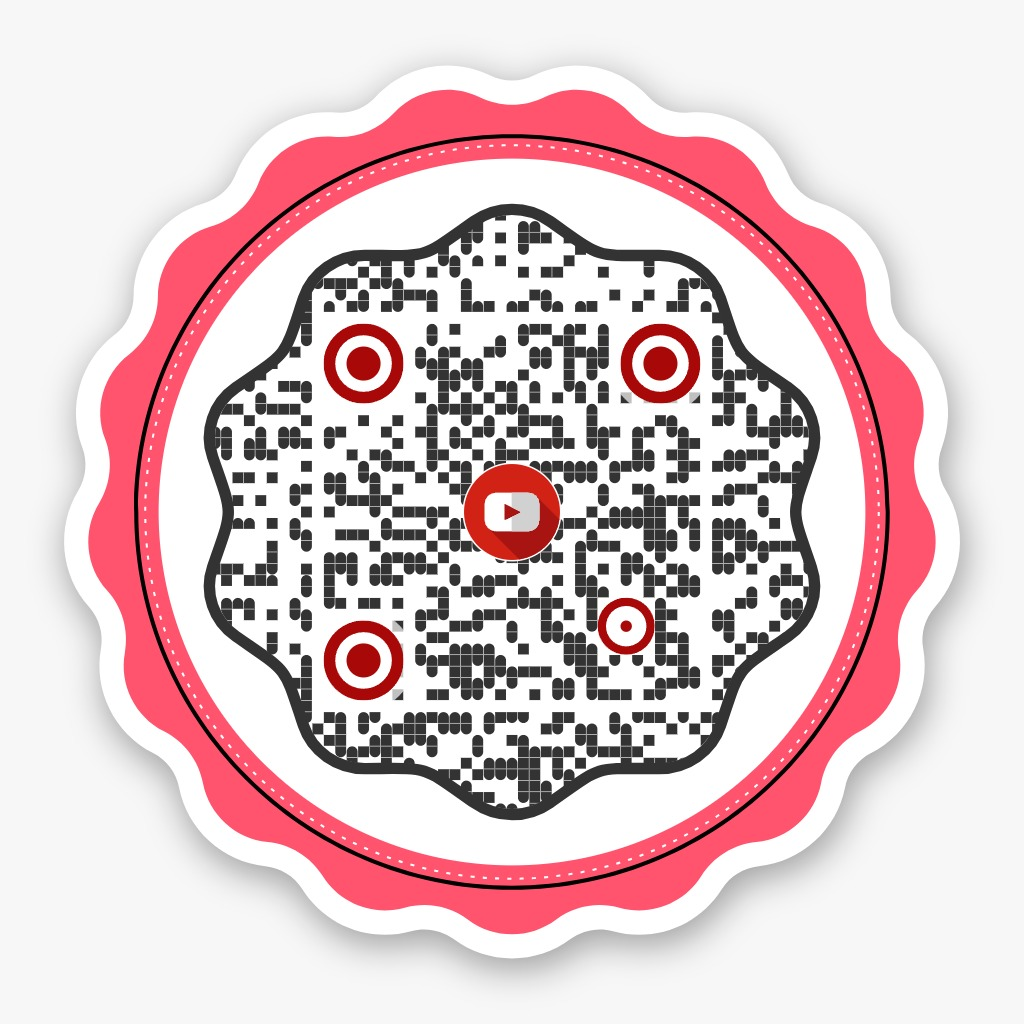
\includegraphics[width=0.4\textwidth]{QRyoutube.jpeg} % <-- QR görselinin adını burada güncelle

\vspace{1em}

{\small
Thank you for listening to our presentation! \\
If you're interested,\\ you can explore more by scanning the QR code.
}
\end{frame}

\end{document}
